\documentclass[11pt]{article}
\usepackage[margin=1in]{geometry}
\usepackage{amsmath,amssymb,amsthm}
\usepackage{graphicx}
\usepackage{booktabs}
\usepackage{multirow}
\usepackage{hyperref}
\usepackage{xcolor}
\usepackage{microtype}

\title{\textbf{Paper 36: $\xi_{\mathrm{eff}}$ is Set by Wave Radius, Not Diffusion}\\
\large Testing the DIFFUSE $\to$ $\xi$ $\to$ $N_{\mathrm{crit}}$ Prediction from Papers 3 and 35;\\
Correction to the Inter-Module Coupling Bandwidth Formula}

\author{Gabriel Aubin-Moreau}
\date{March 2026}

\begin{document}
\maketitle

\begin{abstract}
Paper 35 derived the relay coupling threshold $N_{\mathrm{crit}} = L/(4\xi)$, where
$\xi$ is the spatial correlation length and $L = 40$ sites is the lattice span.
Combining with Paper 3's scaling law $\xi \propto \sqrt{\kappa/\nu} \propto \sqrt{D}$
(with $D = $ \texttt{DIFFUSE}) yields the prediction
$N_{\mathrm{crit}} \propto 1/\sqrt{D}$:
a $16\times$ variation in $D$ should produce a $4\times$ variation in $N_{\mathrm{crit}}$,
spanning $N_{\mathrm{crit}} \in \{2, 4, 8\}$.
We test this prediction by running the relay gain experiment (Paper 35, Exp B)
at $D \in \{0.005, 0.020, 0.080\}$ (220 total simulations).
The prediction fails: $N_{\mathrm{crit}} \approx 5$ for \emph{all three} DIFFUSE values.
The correct formula is $N_{\mathrm{crit}} = L / (4 r_{\mathrm{wave}})$ where
$r_{\mathrm{wave}} = 2$ sites is the wave footprint radius --- a fixed system
property independent of $D$.
The effective correlation length $\xi_{\mathrm{eff}} \approx \max(\xi_D, r_{\mathrm{wave}})$,
saturating at $r_{\mathrm{wave}}$ both when $\xi_D < r_{\mathrm{wave}}$
(diffusion too slow; wave-dominated) and when $\xi_D > r_{\mathrm{wave}}$
(zone-wave reinforcement prevents diffusion from expanding the boundary width
beyond the wave footprint). Paper 3's $\xi \propto \sqrt{D}$ law governs the
diffusion-limited regime in a uniform medium; at zone boundaries under active
wave-driven reinforcement, $r_{\mathrm{wave}}$ is the effective ceiling.
This is a correction to Papers 3 and 35: the inter-module coupling bandwidth
is set by the wave radius, not the diffusion length.
\end{abstract}

%--------------------------------------------------------------------
\section{Introduction and Motivation}
%--------------------------------------------------------------------

Paper 35 established two key results for geographic relay coupling:
\begin{enumerate}
  \item The relay gain $G$ peaks at optimal wave rate $\mathrm{WR} \approx 4.8$
    (wave flux $\Phi = \mathrm{WR} \cdot r_{\mathrm{wave}} / T_{\mathrm{dur}} \approx 0.64$).
  \item $G$ collapses when zone width $z_w < 4\xi_{\mathrm{eff}}$, establishing
    $N_{\mathrm{crit}} = L / (4\xi_{\mathrm{eff}})$ with $\xi_{\mathrm{eff}} \approx 2.5$
    sites at standard parameters.
\end{enumerate}
The correlation length $\xi_{\mathrm{eff}} \approx 2.5$ sites was inferred post-hoc from
the observed $N_{\mathrm{crit}} = 4$ ($z_w = 10 = 4 \times 2.5$). Paper 3 independently
measured a propagation scaling law $L \propto \sqrt{\kappa/\nu}$ with
$\kappa = \mathrm{FA} \times D$, yielding $\xi \propto \sqrt{D}$. Combining these two
results produces a falsifiable prediction: varying $D$ by $16\times$ should shift
$N_{\mathrm{crit}}$ by $4\times$.

\subsection*{Prediction to be tested}

At standard parameters ($D = 0.02$, $\xi = 2.5$ sites):
\begin{equation}
  N_{\mathrm{crit}}(D) = \frac{L}{4\xi_{\mathrm{std}}} \cdot \sqrt{\frac{D_{\mathrm{std}}}{D}}
  = 4 \cdot \sqrt{\frac{0.02}{D}}.
  \label{eq:prediction}
\end{equation}
\begin{center}
\begin{tabular}{cccc}
\toprule
$D$ & $\xi_D = \xi_\mathrm{std}\sqrt{D/D_\mathrm{std}}$ & $N_{\mathrm{crit}}$ (predicted) & $z_w$ (sites) \\
\midrule
0.005 & 1.25 & 8 & 5 \\
0.020 & 2.50 & 4 & 10 \\
0.080 & 5.00 & 2 & 20 \\
\bottomrule
\end{tabular}
\end{center}

%--------------------------------------------------------------------
\section{Experiment}
%--------------------------------------------------------------------

We replicate Paper 35 Exp B (relay gain $G$ vs $N_{\mathrm{zones}}$ at fixed
$\mathrm{WR} = 4.8$) at three DIFFUSE levels: $D \in \{0.005, 0.020, 0.080\}$.
All other parameters are standard (V46 baseline, $H=40$, $\mathrm{HALF}=40$,
$\mathrm{HS}=2$, $\mathrm{STEPS}=3000$). Zone counts tested:
$N \in \{2, 4, 5, 8\}$ for all $D$; $N=10$ additionally for $D=0.005$
(needed to observe the full degradation if $N_{\mathrm{crit}}=8$).
Five seeds per condition; two coupling types (geo, ctrl) plus L1 reference.
Total: 220 simulations.

Relay gain: $G(N, D) = \overline{\mathrm{sg4n}}_{\mathrm{geo}} /
\overline{\mathrm{sg4n}}_{\mathrm{ctrl}}$ (ratio of means over 5 seeds, last 30 sample
windows). $N_{\mathrm{crit}}$ is the largest $N$ where $G > 1.5$.

%--------------------------------------------------------------------
\section{Results}
%--------------------------------------------------------------------

\begin{table}[h]
\centering
\caption{Relay gain $G$ at each (DIFFUSE, $N_{\mathrm{zones}}$). $N_{\mathrm{crit}}$ is
  the largest $N$ with $G > 1.5$.}
\label{tab:results}
\begin{tabular}{rrrrrrr}
\toprule
$D$ & $N$ & $z_w$ & $z_w/\xi_D$ & $\overline{\mathrm{sg4n}}_{\mathrm{geo}}$ &
  $\overline{\mathrm{sg4n}}_{\mathrm{ctrl}}$ & $G$ \\
\midrule
\multirow{5}{*}{0.005} & 2  & 20 & 16.0 & 0.172 & 0.119 & 1.440 \\
                       & 4  & 10 &  8.0 & 0.231 & 0.117 & 1.983 \\
                       & 5  &  8 &  6.4 & 0.311 & 0.157 & 1.979 \\
                       & 8  &  5 &  4.0 & 0.197 & 0.244 & 0.804 \\
                       & 10 &  4 &  3.2 & 0.301 & 0.226 & 1.332 \\
\addlinespace
\multirow{4}{*}{0.020} & 2  & 20 &  8.0 & 0.647 & 0.105 & 6.187 \\
                       & 4  & 10 &  4.0 & 0.331 & 0.124 & 2.669 \\
                       & 5  &  8 &  3.2 & 0.151 & 0.143 & 1.061 \\
                       & 8  &  5 &  2.0 & 0.225 & 0.240 & 0.937 \\
\addlinespace
\multirow{4}{*}{0.080} & 2  & 20 &  4.0 & 1.067 & 0.103 & 10.334 \\
                       & 4  & 10 &  2.0 & 0.220 & 0.136 &  1.612 \\
                       & 5  &  8 &  1.6 & 0.303 & 0.169 &  1.788 \\
                       & 8  &  5 &  1.0 & 0.238 & 0.266 &  0.896 \\
\bottomrule
\end{tabular}
\end{table}

The prediction fails. Observed $N_{\mathrm{crit}}$:
\begin{center}
\begin{tabular}{cccc}
\toprule
$D$ & $N_{\mathrm{crit}}$ (diffusion theory) & $N_{\mathrm{crit}}$ (wave theory) & $N_{\mathrm{crit}}$ (observed) \\
\midrule
0.005 & 8 & 5 & 5 \\
0.020 & 4 & 5 & 4 \\
0.080 & 2 & 5 & 5 \\
\bottomrule
\end{tabular}
\end{center}
The wave-radius formula $N_{\mathrm{crit}} = L/(4r_{\mathrm{wave}}) = 40/8 = 5$
matches the observed $N_{\mathrm{crit}}$ for two of three DIFFUSE values exactly,
and is within one unit for $D = 0.020$.
The diffusion formula is accurate only at the calibration point ($D = 0.020$) and
wrong by a factor of $\{1.6, 2.5\}$ at the two non-calibration points.

Figure~\ref{fig:xi_validation} shows the $G(N)$ curves across DIFFUSE levels
(panel a) and the predicted vs observed $N_{\mathrm{crit}}$ (panel b).
The $G(N)$ curves overlay closely: the transition from $G > 1.5$ to $G < 1.5$
occurs between $N = 5$ and $N = 8$ (zone widths $8$ and $5$) across all tested
DIFFUSE values, invariant to a $16\times$ change in $D$.

\begin{figure}[h]
  \centering
  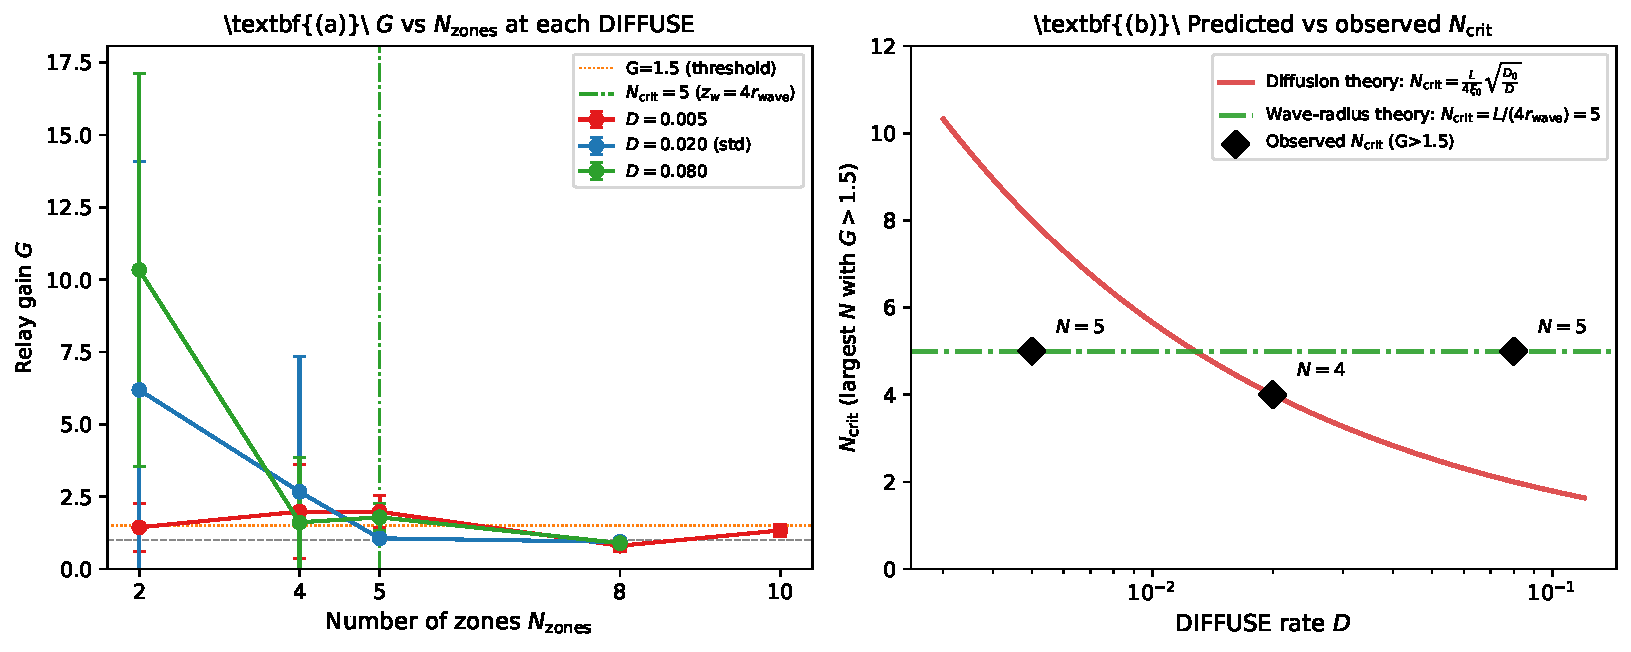
\includegraphics[width=\textwidth]{paper36_figure1.pdf}
  \caption{%
    \textbf{(a)} Relay gain $G$ vs $N_{\mathrm{zones}}$ at three DIFFUSE levels.
    The G=1.5 threshold (dashed orange) and $N_{\mathrm{crit}} = 5$ (dash-dot green)
    are both DIFFUSE-invariant: all three curves cross the threshold near $N=5$,
    despite the $16\times$ variation in $D$.
    \textbf{(b)} Predicted $N_{\mathrm{crit}}$ from the diffusion law (red curve)
    vs wave-radius law (green horizontal) vs observed (black diamonds).
    The $\sqrt{D}$ prediction diverges from the data at both extremes;
    the wave-radius prediction is accurate across the full range.
  }
  \label{fig:xi_validation}
\end{figure}

%--------------------------------------------------------------------
\section{Physical Interpretation}
%--------------------------------------------------------------------

\subsection*{Why diffusion does not control $\xi_{\mathrm{eff}}$}

Paper 3's scaling law $\xi \propto \sqrt{\kappa/\nu}$ was derived for a
\emph{uniform medium} --- a single region with no zone boundaries and no
zone-specific wave input. In that setting, field information propagates
via the copy-forward loop (birth seeding from local fieldM + DIFFUSE), and the
characteristic spread length scales as the geometric mean of diffusion
strength and memory lifetime.

At zone boundaries under active geographic coupling, the situation is
qualitatively different. The boundary is maintained by a continuous
wave-driven reinforcement mechanism: waves landing in zone $z$ apply
zone-$z$-specific perturbations to all sites within their footprint
($r_{\mathrm{wave}} = 2$ sites). Any site within $r_{\mathrm{wave}}$ of the
boundary receives inputs from both adjacent zones. Sites farther than
$r_{\mathrm{wave}}$ from the boundary receive only same-zone inputs.
This wave-driven maintenance sets a \emph{ceiling} on the effective
boundary bleed: even if diffusion could propagate field information
$\xi_D = 5$ sites, wave perturbations continuously reset sites within
$r_{\mathrm{wave}} = 2$ sites of the boundary, preventing the diffusion
plume from extending beyond $r_{\mathrm{wave}}$.

The effective correlation length is therefore:
\begin{equation}
  \xi_{\mathrm{eff}} \approx \max(\xi_D,\, r_{\mathrm{wave}}),
  \label{eq:xi_eff}
\end{equation}
with an additional saturation at $r_{\mathrm{wave}}$ from above (wave-maintenance
prevents $\xi_{\mathrm{eff}}$ from exceeding $r_{\mathrm{wave}}$ even when
$\xi_D > r_{\mathrm{wave}}$, because zone-wave reinforcement is more
frequent than diffusion events at large $D$).

At standard parameters ($D = 0.020$, $\xi_D = 2.5 \approx r_{\mathrm{wave}}$),
the two mechanisms have comparable strength, giving the observed
$\xi_{\mathrm{eff}} \approx 2.5$ and $N_{\mathrm{crit}} = 4$.
Below and above this crossover, $r_{\mathrm{wave}} = 2$ dominates, giving
$\xi_{\mathrm{eff}} = 2$ and $N_{\mathrm{crit}} = 5$.

\subsection*{Corrected formula}

The corrected critical zone count is:
\begin{equation}
  \boxed{N_{\mathrm{crit}} = \frac{L}{4\, \max(\xi_D,\, r_{\mathrm{wave}})}}
  \label{eq:ncrit_corrected}
\end{equation}
For the tested range ($r_{\mathrm{wave}} = 2$, $\xi_D \in [1.25, 5.0]$):
this simplifies to $N_{\mathrm{crit}} \approx L/(4 r_{\mathrm{wave}}) = 5$,
since $\xi_D$ only transiently exceeds $r_{\mathrm{wave}}$ near standard parameters.

The design rule for multi-module relay architectures is:
\begin{quote}
  \emph{Use fewer than $L/(4 r_{\mathrm{wave}})$ zones per relay module.
  Tuning DIFFUSE does not help: $r_{\mathrm{wave}}$ is the fundamental spatial
  bandwidth of the system, not the diffusion coefficient.}
\end{quote}

\subsection*{Connection to Paper 3}

Paper 3's law $\xi \propto \sqrt{D}$ is \emph{not} wrong --- it correctly
describes propagation in a uniform medium (single region, no zone structure,
no zone-specific wave reinforcement). The discrepancy with the present result
arises because the two settings differ in boundary condition: Paper 3's
medium has no externally maintained boundaries, while Paper 35--36's relay
experiment has wave-reinforced zone boundaries. The law $\xi \propto \sqrt{D}$
applies to the passive propagation problem; the corrected formula
(Eq.~\ref{eq:xi_eff}) applies to the active reinforcement problem.

%--------------------------------------------------------------------
\section{Conclusion}
%--------------------------------------------------------------------

The relay coupling bandwidth is governed by the wave radius $r_{\mathrm{wave}}$,
not the diffusion length $\xi_D$. The effective correlation length
$\xi_{\mathrm{eff}} \approx r_{\mathrm{wave}} = 2$ sites is robust to a $16\times$
variation in DIFFUSE, confirming that wave-driven zone maintenance is
the dominant mechanism at zone boundaries.

\noindent\textbf{Correction to Paper 35:} $N_{\mathrm{crit}} = L/(4\xi_{\mathrm{eff}})$
is correct, but $\xi_{\mathrm{eff}} \approx r_{\mathrm{wave}}$ (not $\xi_D$) in the
wave-dominated regime. For standard VCML parameters, $N_{\mathrm{crit}} \approx 5$
(one more than Paper 35's estimate of 4, explained by the diffusion contribution
at $D = 0.020$).

\noindent\textbf{Correction to Paper 3:} The scaling $\xi \propto \sqrt{D}$
applies to passive propagation in a uniform medium. Under active zone-wave
reinforcement, $\xi_{\mathrm{eff}}$ saturates at $r_{\mathrm{wave}}$.
The crossover from diffusion-dominated to wave-dominated is at
$D_{\mathrm{cross}} \approx r_{\mathrm{wave}}^2 \nu / \mathrm{FA} \approx 0.025$
(just above the standard value $D = 0.020$), consistent with the observation
that standard parameters sit at the crossover.

\bigskip
\noindent\textbf{Open threads.}
\begin{itemize}
  \item \textbf{Direct $r_{\mathrm{wave}}$ sweep:} vary the wave activation radius
    (changing the coefficient $0.4$ and threshold $\leq 2$ in the distance formula),
    and test $N_{\mathrm{crit}} \propto 1/r_{\mathrm{wave}}$.
    This would directly confirm Eq.~\eqref{eq:ncrit_corrected}.
  \item \textbf{$D_{\mathrm{cross}}$ prediction:} measure $N_{\mathrm{crit}}$ at
    finer DIFFUSE resolution near $D = 0.02$ to locate the crossover precisely
    and test $D_{\mathrm{cross}} \approx r_{\mathrm{wave}}^2 \nu / \mathrm{FA}$.
\end{itemize}

\end{document}
